% Déclaration du type de document (report, book, paper, etc...)
\documentclass[a4paper, 10pt]{article}

% Package pour avoir Latex en français
\usepackage[utf8]{inputenc}
\usepackage[T1]{fontenc}

% Quelques packages utiles
\usepackage{listings} % Pour afficher des listings de programmes
\usepackage{graphicx} % Pour afficher des figures
\usepackage{amsthm}   % Pour créer des théorèmes et des définitions
\usepackage{amsmath}
\usepackage{microtype} % Optical margins FTW
\usepackage{url}
\usepackage{booktabs} % Allows the use of \toprule, \midrule and \bottomrule in tables for horizontal lines
\usepackage{siunitx}
\usepackage{floatrow}
\usepackage[justification=centering]{caption}
\usepackage{subcaption}
\usepackage{fullpage}
\usepackage{lipsum}
\usepackage{cite}
\usepackage{mhchem}
\usepackage[acronym,smallcaps]{glossaries}
\graphicspath{{media/}}
\setlength\parindent{0pt} % Removes all indentation from paragraphs

\author{Antoine Albertelli \texttt{} \and
        Salah-Eddine Missri \texttt{} \and
        Patrick Spieler \texttt{}}
\title{Asynchronous odometry based dead reckoning localisation system for Eurobot}

\begin{document}
\maketitle
\hrulefill
\tableofcontents
\hrulefill

\section*{Abstract}
\lipsum[1]

\section{Conventions}
\begin{figure}[h]
    \begin{center}
        \includegraphics[width=0.8\textwidth]{table}
        \caption{Coordinate system of the robot on the Eurobot table}
        \label{fig:coordinates}
    \end{center}
\end{figure}

The global coordinate system is defined according to the game table referential frame (fig. \ref{fig:coordinates}).
The coordinate system is in a direct base.
It is expressed in standard units (\si{\meter} and \si{\radian}).
It doesn't change when changing team color.

The input of the algorithm are the following:
\begin{itemize}
    \item $\Delta R$ and $\Delta L$ are the right and left change in position difference in encoder ticks.
    \item $\phi_t^R$ and $\phi_t^L$ are the right and left encoder angular position at time $t$
    \item $r_R$ and $r_L$ are the right and left wheel radius in \si{\meter}.
    \item $\lambda = \frac{r_L}{r_R}$ is defined as the wheel correction factor and is used in the calibration process.
    \item $b$ is the wheelbase of the robot (distance between the wheels) in \si{\meter}.
    \item $N$ is the number of encoder ticks per revolution of the wheel and is defined as $2^{16}$.
\end{itemize}


\section{Update algorithm}
Since we have a distributed architecture on our robots, each wheel of the base is handled by a separate node that communicates with a master node.
The master node runs the pose estimation using the odometry data from the two wheels, but since the encoders are not sampled and at the same time and the samples are not received at the same time, we can't apply the standard dead reckoning formulas.

\subsection{Dealing with asynchronicity by decoupling the wheels}
A simple but naive approach is to only update one wheel at a time, so we assume that only the wheel we are updating moved while the other one stayed still.
That means if we just received $\Delta L$, we assume that $\Delta R$ is zero.

\begin{figure}[h]
    \begin{center}
        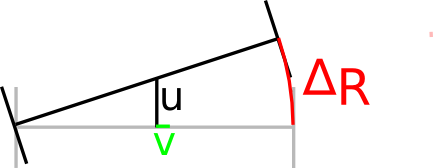
\includegraphics[width=0.4\textwidth]{algorithm.png}
        \caption{Visual explanation of the algorithm}
    \end{center}
\end{figure}

We start by computing the difference in heading $\Delta \theta$:
\begin{equation}
    \Delta \theta = \frac{\Delta R - \Delta L}{b}
\end{equation}

Then we can compute the robot movement :
\begin{equation}
    \begin{pmatrix}
        u\\v
    \end{pmatrix}
    =
    \frac{b}{2}
    \begin{pmatrix}
        \sin \Delta \theta\\1 - \cos \Delta \theta
    \end{pmatrix}
    \approx
    \frac{b}{2}
    \begin{pmatrix}
        \Delta \theta\\ 0
    \end{pmatrix}
\end{equation}

We will then transpose those displacement vector in the global space ($\theta$ is the heading of the robot):
\begin{equation}
    \begin{pmatrix}
        \Delta x\\\Delta y
    \end{pmatrix}
    =
    \begin{pmatrix}
        \cos\theta \\-\sin\theta
    \end{pmatrix}
    u
\end{equation}

Finally, integrate the change into the robot position:
\begin{equation}
    \begin{pmatrix}
        x_{k+1}\\
        y_{k+1}\\
        \theta_{k+1}
    \end{pmatrix}
    =
    \begin{pmatrix}
        x_{k}\\
        y_{k}\\
        \theta_{k}
    \end{pmatrix}
    +
    \begin{pmatrix}
        \Delta x\\\Delta y\\\Delta \theta
    \end{pmatrix}
\end{equation}

This approach yields unsatisfactory results as the error accumulates quickly.

\subsection{Encoder Interpolation}
A better way of dealing with asynchronicity is to set one of the two wheels sample as reference, then interpolate or predict the value of the other wheel at the time of measurement of the reference wheel.

To achieve this we use the previous samples of an encoder wheel and fit a polynomial curve to them.
Assuming a constant acceleration motion model of the wheel, fitting a second order polynomial to the last three samples should suffise.

For any arbitrary $t$, $t_0 < t_1 < t_2$, the encoder position can be expressed as:
\begin{equation}
    \phi_t
    = \gamma + \beta (t - t_2) + \alpha (t - t_2)^2
    =
    \begin{pmatrix}
        (t - t_2)^2 \\
        t - t_2 \\
        1
    \end{pmatrix}^T
    \begin{pmatrix}
        \alpha \\
        \beta \\
        \gamma
    \end{pmatrix}
    \label{eqn:encoder_parabola}
\end{equation}

Where $\gamma$, $\beta$ and $\alpha$ are the parabolic motion parameters obtained from the samples by simply solving
\begin{equation}
    \begin{pmatrix}
        \phi_{t_0} \\
        \phi_{t_1} \\
        \phi_{t_2}
    \end{pmatrix}
    =
    \begin{pmatrix}
        t_0^2 & t_0 & 1 \\
        t_1^2 & t_1 & 1 \\
        t_2^2 & t_2 & 1
    \end{pmatrix}
    \begin{pmatrix}
        \alpha \\
        \beta \\
        \gamma
    \end{pmatrix}
    \iff
    \begin{pmatrix}
        \phi_{t_0} \\
        \phi_{t_1} - \phi_{t_0} \\
        \phi_{t_2} - \phi_{t_0}
    \end{pmatrix}
    =
    \begin{pmatrix}
        t_0^2         & t_0       & 1 \\
        t_1^2 - t_0^2 & t_1 - t_0 & 0 \\
        t_2^2 - t_0^2 & t_2 - t_0 & 0
    \end{pmatrix}
    \begin{pmatrix}
        \alpha \\
        \beta \\
        \gamma
    \end{pmatrix}
\end{equation}
With $\phi_{t_0}$, $\phi_{t_1}$ and $\phi_{t_2}$ the last three samples recorded at time $t_0$, $t_1$ and $t_2$ respectively.

This can be simplified by assuming WLOG that $t_0 = 0$ - we can do this because the system is shift invariant - which yields
\begin{equation}
    \begin{pmatrix}
        \alpha \\
        \beta \\
        \gamma
    \end{pmatrix}
    =
    \begin{pmatrix}
        0 & \frac{ -1}{t_1 (t_2 - t_1)} & \frac{ -1}{t_2 (t_1 - t_2)} \\
        0 & \frac{t_2}{t_1 (t_2 - t_1)} & \frac{t_1}{t_2 (t_1 - t_2)} \\
        1 & 0 & 0
    \end{pmatrix}
    \begin{pmatrix}
        \phi_{t_0} \\
        \phi_{t_1} - \phi_{t_0} \\
        \phi_{t_2} - \phi_{t_0}
    \end{pmatrix}
    \label{eqn:param_parabola}
\end{equation}

Computing $\phi_t$ comes down to computing the parabola parameters with (\ref{eqn:param_parabola}) then inject the result in (\ref{eqn:encoder_parabola}).
So now, we can generate an interpolated sample at any time $t$, which means that our asynchronous system can be reduced down to a synchronous one.
We can now apply the differential base odometry formulas.

\subsection{Differential base odometry}
NB: For abreviation, we will write $\Delta f_{a,b} = f_a - f_b$.

In the case of the differential base, the odometry formulas are
\begin{equation}
\left\{
\begin{array}{lr}
    \Delta s_{t,t+\Delta t} = \frac{1}{2} (r_R \Delta \phi_{t,t+\Delta t}^R + r_L \Delta \phi_{t,t+\Delta t}^L) \\
    \Delta \theta_{t,t+\Delta t}  = \frac{1}{b} (r_R \Delta \phi_{t,t+\Delta t}^R - r_L \Delta \phi_{t,t+\Delta t}^L)
\end{array}
\right.
\end{equation}
Where $\Delta s$ denotes forward motion and $\Delta \theta$ denotes rotational motion.
\\
The kinematics of the robot can be modeled using the forward velocity $v(\tau)$ and the rotational velocity $\omega(\tau)$.
The integration time being small, we can assume that $v(\tau)$ and $\omega(\tau)$ remain constant for $\tau \in [t, t+\Delta t]$ and are given by:
\begin{equation}
\left\{
\begin{array}{lcl}
    \Delta s_{t,t+\Delta t} &=& v(\tau) \cdot \Delta t \\
    \Delta \theta_{t,t+\Delta t} &=& \omega(\tau) \cdot \Delta t
\end{array}
\right.
\iff
\left\{
\begin{array}{lcl}
    v(\tau) &=&  \frac{\Delta s_{t,t+\Delta t}}{\Delta t} \\
    \omega(\tau) &=& \frac{\Delta \theta_{t,t+\Delta t}}{\Delta t}
\end{array}
\right.
\label{eqn:discrete_speeds}
\end{equation}

Therefore the kinematics of the robot in a cartesian frame are given by:
\begin{equation}
\left\{
\begin{array}{lcl}
    \dot x &=& v(\tau) \cos(\theta(\tau)) \\
    \dot y &=& v(\tau) \sin(\theta(\tau)) \\
    \dot \theta &=& \omega(\tau)
\end{array}
\right.
\end{equation}

From this, the robot's pose can be computed through integration:
\begin{equation}
\left\{
\begin{array}{lcl}
    \Delta x_{t,t+\Delta t} = \int_t^{t+\Delta t} v(\tau) \cos(\theta(\tau)) d\tau \\
    \Delta y_{t,t+\Delta t} = \int_t^{t+\Delta t} v(\tau) \sin(\theta(\tau)) d\tau \\
    \Delta \theta_{t,t+\Delta t} = \int_t^{t+\Delta t} \theta(\tau) d\tau \\
\end{array}
\right.
\end{equation}

We can derive the exact velocity model through continuous time-domain integration:
\begin{equation}
\left\{
\begin{array}{lcl}
    \Delta x_{t,t+\Delta t} = \frac{v}{\omega} (\sin(\theta_{t}) - \sin(\theta_{t+\Delta t})) \\
    \Delta y_{t,t+\Delta t} = - \frac{v}{\omega} (\cos(\theta_{t}) - \cos(\theta_{t+\Delta t})) \\
    \Delta \theta_{t,t+\Delta t} = \omega \Delta t \\
\end{array}
\right.
\end{equation}

However, we are constrained to work in discrete time-domain, so we use second order Runge-Kutta to integrate:
\begin{equation}
\left\{
\begin{array}{lcl}
    \Delta x_{t,t+\Delta t} = v \cos(\theta + \omega \frac{\Delta t}{2}) \Delta t \\
    \Delta y_{t,t+\Delta t} = v \sin(\theta + \omega \frac{\Delta t}{2}) \Delta t \\
    \Delta \theta_{t,t+\Delta t} = \omega \Delta t \\
\end{array}
\iff
\begin{array}{lcl}
    \Delta x_{t,t+\Delta t} = \Delta s_{t,t+\Delta t} \cos(\theta + \frac{\Delta \theta_{t,t+\Delta t}}{2}) \\
    \Delta y_{t,t+\Delta t} = \Delta s_{t,t+\Delta t} \sin(\theta + \frac{\Delta \theta_{t,t+\Delta t}}{2}) \\
    \Delta \theta_{t,t+\Delta t} = \Delta \theta_{t,t+\Delta t} \\
\end{array}
\right.
\end{equation}

Using (\ref{eqn:discrete_speeds}) and the definition of $\phi_t$: $\phi_t^R = \frac{2\pi}{N} \Delta R$, the update step comes down to computing
\begin{equation}
\left\{
\begin{array}{lcl}
    \Delta s_{t,t+\Delta t} = \frac{\pi}{N} (r_R \Delta R_{t,t+\Delta t} + r_L \Delta L_{t,t+\Delta t}) \\
    \Delta \theta_{t,t+\Delta t}  = \frac{2\pi}{bN} (r_R \Delta R_{t,t+\Delta t} - r_L \Delta L_{t,t+\Delta t}) \\
    x_{t+\Delta t} = x_t + \Delta s_{t,t+\Delta t} \cos(\theta + \frac{\Delta \theta_{t,t+\Delta t}}{2}) \\
    y_{t+\Delta t} = y_t + \Delta s_{t,t+\Delta t} \sin(\theta + \frac{\Delta \theta_{t,t+\Delta t}}{2}) \\
    \theta_{t+\Delta t}  = \theta_t + \Delta \theta_{t,t+\Delta t} \\
\end{array}
\right.
\end{equation}


\section{Accounting for mechanical tolerances}
In the previous sections we supposed that the two measuring wheels were perfectly identical, with the same tick to meter ratio.
However, in the real world, manufacturing tolerances are not perfect and wheel diameters can vary quite a lot.
Using the ISO 2768-f specification on a \SI{40}{\milli\meter} wheel yields a maximum tolerance of $\pm \SI{0.2}{\milli\meter}$.
This means that between both wheels the maximum relative error is $\frac{\Delta R}{R} = \frac{2 \cdot 0.2}{40} = 1\% $.

How does this error translate into robot trajectory ?
Well when the robot thinks it is doing a straight line, it will actually be turning in a slight circle.

Each will will run on a cirlcle of radius $R$.
The distance between the wheels is fixed so :
\begin{equation*}
    R_1 - R_2 = T
\end{equation*}

The robot turned of a given angle $\alpha$ so :
\begin{equation*}
    R_1 \alpha = \lambda R_2 \alpha
\end{equation*}

Therefore:
\begin{equation*}
    (T + R_2) \alpha = \lambda R_2 \alpha
\end{equation*}

And finally we got the radius of the trajectory :
\begin{equation*}
    R = T \left(\frac{1}{\lambda - 1}  + \frac{1}{2}\right)
\end{equation*}

Plugging reasonable parameters for Eurobot ($\lambda=1+0.1\%$, $T = \SI{0.2}{\meter}$), we obtain a radius $R = \SI{300}{\meter}$.
Such a big radius might seem indistinguishable from a straight line, but this is not the case.
To show this, let's compute the lateral deviation on a full table crossing (\SI{2.5}{\meter}):
\begin{equation*}
    \Delta x = \left( 1 - \cos \frac{2.5}{300} \right) \cdot \SI{300}{\meter} \approx \SI{1}{\centi\meter}
\end{equation*}


Compensating this effect is trivial.
Simply apply the correction factor $\lambda$ to the right wheel input before computing odometry:
\begin{equation}
    \Delta R' = \lambda \Delta R
\end{equation}

\section{Calibration procedure}
Since we already shown that mechanical construction is not to be relied on, we have to calibrate the parameters experimentally.
The order of parameter determination matters, since they are inter dependent.
The parameters are:
\begin{itemize}
    \item $\lambda$ (wheel correction factor)
    \item $N$ (Encoder ticks per millimeter)
    \item $T$ (Distance between both wheels)
\end{itemize}

\subsection{Wheel correction factor}
Start with $\lambda=1$.
The wheel correction factor measurement is as follows:

\begin{enumerate}
    \item The robot takes its reference by pushing against a reference plate.
        Wheel positions are stored ($R_i$ and $L_i$ for right and left respectively).
    \item Go away from the reference plate, just enough to allow rotation of the robot.
    \item The robot repeats the following sequence.
        The recommended way is to start with few iterations then increase until enough precision is achieved.
        \begin{enumerate}
            \item Go forward by at least \SI{1.5}{\meter} (more is better).
            \item Rotate by \SI{180}{\degree}.
            \item Go forward by the same distance as before
            \item Rotate by \SI{-180}{\degree}.
                The sign of the rotation matters:
                Since the track of the robot is not calibrated yet, turning in opposite directions effectively cancels the rotation error.
        \end{enumerate}
    \item The robot takes it reference, by pressing against the reference plate again.
        Wheel position is stored again and noted $R_f$ and $L_f$.
\end{enumerate}

The correction factor can now be computed as :
\begin{equation}
    \lambda = \frac{(R_i - L_i) - (R_f - L_f)}{(R_i + L_i) - (R_f + L_f)}
\end{equation}

\subsection{Encoder ticks per meter}
This one is the least precise part of the calibration procedure.
Fortunately it is the part that has the least influence on the end result.
When using wheels without O-Rings, this part can be skipped.

Start with the theoretical value for $N$.
Then ask the robot to go forward by a distance $d$.
The longest is better, but be sure to do it on a clean, flat surface.
Measure $d'$ the distance the robot travelled.
The compensated value is :
\begin{equation}
    N' = N \frac{d}{d'}
\end{equation}

One iteration should be enough for this calibration if done correctly.



\subsection{Wheel track}
The calibration of the wheel track is pretty straightforward.
Start with the nominal value.
\begin{itemize}
    \item The robot takes a reference against a plate and sets $\theta = 0$.
    \item The robot goes a bit away from the reference plate to allow free rotation.
    \item The robot makes $k$ full turns.
        Start with a low turn count and increase until necessary precision is reached.
    \item The robot aligns itself against the reference plate again.
    \item The angle measured by the robot is now the rotation error ($\Delta \theta$).
\end{itemize}
Now the corrected track value can be set using equation \ref{eqn:track-correction}.
Repeat as many times as needed for the desired precision value.
\begin{equation}
    T' = T \left(1 + \frac{\Delta \theta}{k \cdot 2\pi}\right)
    \label{eqn:track-correction}
\end{equation}

\end{document}
